\section{循环反应器}


\begin{frame}[t]
    \frametitle{循环反应器}
    \begin{figure}
        \centering
        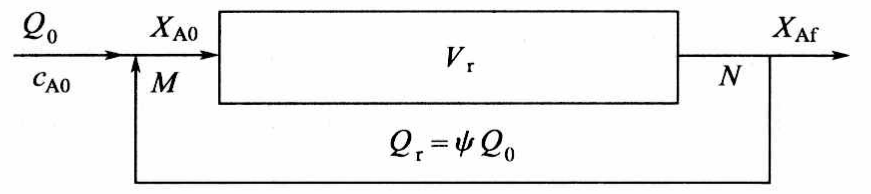
\includegraphics[width=.75\linewidth]{figs/fig4.6.png}
    \end{figure}
    \only<1>{
    \begin{itemize}
        \item 物料处理量$=?$
        \item 入口转化率$=?$
    \end{itemize}
    }
    \only<2>{
        反应器物料处理量
        \[
            Q_0 + Q_\mathrm{r} = (1 + \varphi) Q_0
        \]
        对M点作A的物料衡算
        \[
            Q_{0} c_{\mathrm{A} 0}+\varphi Q_{0} c_{\mathrm{A} 0}(1-X_{\mathrm{Af}})=(1+\varphi) Q_{0} c_{\mathrm{A} 0}(1-X_{\mathrm{A} 0})
        \]
        \[
            X_{\mathrm{A} 0}=\frac{\varphi  X_{\mathrm{Af}}}{1+\varphi}
        \]
    }
    \only<3>{
        \[
        V_{\mathrm{r}}=(1+\varphi) Q_{0} c_{\mathrm{A} 0} \int_{\frac{\varphi X_{\mathrm{Af}}}{1+\varphi}}^{X_{\mathrm{Af}}} \frac{\mathrm{d} X_{\mathrm{A}}}{(-\mathscr{R}_{\mathrm{A}})}
    \]
    \begin{itemize}
        \item 当$\varphi \to  0$时，$X_{\mathrm{A0}}=0$，$V_{\mathrm{r}}=(1+\varphi) Q_{0} c_{\mathrm{A} 0} \int_{0}^{X_{\mathrm{Af}}} \frac{\mathrm{d} X_{\mathrm{A}}}{(-\mathscr{R}_{\mathrm{A}})}$
        \item 当$\varphi \to \infty $时，$X_{\mathrm{A0}} \to X_{\mathrm{Af}}$，相当于恒定转化率$X_{\mathrm{Af}}$下操作的釜式反应器。
    \end{itemize}
    }
\end{frame}

